\documentclass[10pt]{article}
\usepackage[a4paper,margin=2.6cm]{geometry}
\usepackage{graphicx}
\usepackage{array}
\usepackage{booktabs}
\usepackage{amsmath}
\usepackage{amssymb}
\usepackage[hidelinks]{hyperref}
\usepackage{xcolor}
\definecolor{ink2}{HTML}{6F6E66}
% \S (section sign) defaults to the TS1 companion font, which this TeX
% installation only has as a 600 dpi bitmap; the OMS symbol font has the
% same glyph as a Type 1 outline, so every \S here is set from it.
\DeclareTextSymbolDefault{\textsection}{OMS}
\graphicspath{{figs/}}
\setlength{\parskip}{2pt}
\renewcommand{\topfraction}{0.9}
\renewcommand{\bottomfraction}{0.7}
\renewcommand{\textfraction}{0.1}
\renewcommand{\floatpagefraction}{0.7}

\title{Earth-State Embeddings:\\
\large a self-supervised codec of the North Atlantic, its transport read-out,\\
and what a transformer forecasts from it}
\author{blauewelt/earth --- technical report}
\date{18 September 2026}

\begin{document}
\maketitle

\begin{abstract}
We compress the observed state of each North Atlantic grid cell --- ocean
reanalysis, Argo climatology, wind stress, sea-surface temperature --- into a
32-dimensional embedding with a self-supervised per-pixel codec, and train a
transformer to predict the embedding forward at five-day cadence.
\textbf{Codec.} Read out by an attention head over the individual pixels of
the $26.5^\circ$N section, the frozen embeddings predict RAPID overturning
transport at $r=0.67$ (two codec seeds, year-blocked k-fold); the same head
fed raw section values reaches $0.66$, so the representation adds nothing
measurable for the current-state read-out. Wind stress accounts for most
monthly skill (a wind-only ridge reaches $0.53$); the 16 Argo levels move
skill to the density-driven MOVE transport at $16^\circ$N; neither codec
capacity ($0.92$M to $40.7$M) nor training length (50k to 1M steps) moves the
probe. \textbf{Forecaster.} Under a training pool that excludes every window
touching a held-out year, stage-2 heads from 7.6M to 400M parameters reach
their best held-out one-step loss inside the first $\sim$2{,}000 of 200{,}000
steps and worsen thereafter, the best level lying in $0.58$--$0.62$ of the
persistence error across a $53\times$ span in capacity. Rolled twelve months
from held-out starts, the 206.7M head's field anomaly correlation decays from
$0.61$ at five days to $0.41$ at ten, $\approx 0.1$ from two months on and
$-0.03$ at a year; it beats raw persistence at every lead but the last and
damped persistence at none. Its squared-error score is negative (mean MSSS
$-0.44$ against climatology) because it emits anomalies at 78\% amplitude at
10\% correlation --- an identity reproduces all 73 leads to $0.0135$, and the
same states rescaled would score $\approx +0.02$. Skill that survives past a
few pentads lives in sea-surface temperature; 32 of 40 channels score nothing
at any lead. A 200-mode linear inverse model fitted to the same field and
rolled from the same starts is less correlated than the head at five and ten
days and more correlated at every lead from fifteen days to a year ($0.26$
at 90 days, $0.18$ at 365), with a squared-error score that stays positive
throughout. Heads of 7.6M and 40.4M parameters rolled through the same
battery have the same mean correlation as the 206.7M head ($0.103$, $0.104$,
$0.105$); their squared-error scores differ ($-0.18$, $-0.26$, $-0.44$) only
through an emitted amplitude that grows with width, and the smallest head
does not decay through zero, holding $\approx 0.11$ from two months to a
year. Transport at $26.5^\circ$N shows no measurable skill at roughly
nine effective starts. Every rolled number is a single seed.
\textbf{Design.} From these constraints we specify the next codec and
forecaster (\S\ref{sec:design}). Both stages sample the same space--time
hourglass --- a learnable past cone as input, its point mirror as the
forecast target --- the codec over raw values at up to six pentads, the
forecaster over the codec's embeddings at log-spaced lags to two years. The
forecaster is a residual on a contractive linear propagator initialised from
the linear inverse model, trained on direct multi-lead targets under a
decoupled Gaussian likelihood, and every choice is tied to the comparison on
the dense field that would accept or reject it.
\end{abstract}

\section{Data}\label{sec:data}

The working tensor covers $0$--$70^\circ$N, $100^\circ$W--$20^\circ$E on a
$0.25^\circ$ grid ($281\times481$ cells, 86{,}698 ocean) at five-day cadence
from 1982-01 to 2024-12 (3{,}142 bins), with 40 channels per cell: surface
current speed, log mixed-layer depth and sea-surface height from the GLORYS
reanalysis; temperature and salinity at 16 pressure levels from the
Roemmich--Gilson Argo climatology (native $1^\circ$, monthly, from 2004);
NCEP Reanalysis-1 wind stress and its within-bin variability (four
channels); OISST sea-surface temperature. Channels absent before their record
begins enter as missing tokens. Earlier codec generations used $1^\circ$
monthly tensors with 12--25 channels, on the same window or globally; they
are identified by channel count below. The transport truth is the RAPID-MOCHA
overturning at $26.5^\circ$N (2004--), deseasonalised; MOVE at $16^\circ$N is
a second target. Everything cited here --- tensors, weights, result bundles
--- is public (Appendix~\ref{app:avail}).

\section{The codec and its read-outs}\label{sec:codec}

\paragraph{Model.} A masked autoencoder over one pixel's channels at one time
bin produces a $d_z$-dimensional embedding; a $3\times3$-patch variant sees
the pixel's neighbours. The working codec on the $0.25^\circ$ pentad tensor
is 512-wide, 12 layers, decoder width 256, $d_z{=}32$, patch 1, 37.976M
parameters, trained 200k steps at batch 512 with 2009, 2017 and 2023 held out
of training and of the anomaly statistics. Embeddings are probed for
transport with a year-blocked k-fold: a ridge on the section-mean embedding
(\emph{pooled}), or an attention head over the section's individual pixels
(\emph{unpooled}). Field reconstruction is scored as the percentage
improvement over persistence, one bin ahead.

\paragraph{What moves the transport read-out.}
Figure~\ref{fig:kfold} is the pooled ranking across generations. Adding wind
stress to a 12-channel tensor takes the pooled probe from $0.31$ to $0.60$; a
wind-only ridge with no embedding reaches $0.531$ on the $1^\circ$ tensors
and $0.568$ on the $0.25^\circ$ one, so most monthly skill at $26.5^\circ$N
is Ekman physics. Training on the global ocean instead of the window costs
the Atlantic read-out nothing ($0.602$ against $0.604$). Bottleneck width
matters little for reconstruction (saturating by $d_z{=}16$--$32$) and peaks
at $d_z{=}64$ for the probe, turning over at 128 against $\sim$220 truth months
per fold. On the $0.25^\circ$ tensor a 0.92M pilot reads $0.620$ and the 40.7M
codec $0.631$ --- $44\times$ the parameters buys $+0.011$, inside seed noise
($\pm0.05$ on the pooled probe) --- and a codec trained from 50k to one
million steps is flat from the first probe to the last. Neither capacity nor
training length is what stands between this codec and a better transport
number.

\begin{figure}[t]
\centering
\includegraphics[width=0.72\linewidth]{fig_kfold.pdf}
\caption{Pooled k-fold correlation with monthly deseasonalised RAPID
transport by codec generation. Blue: the 12-channel width sweep; orange: with
wind stress; green: 24--25 channels with 8 Argo levels; violet: the
$0.25^\circ$ tensor with 16 levels and SSH at two capacities.\label{fig:kfold}}
\end{figure}

\paragraph{Pooling was hiding the signal, and the codec is not what
recovers it.} The same frozen embeddings read three ways
(Figure~\ref{fig:ladder}): an MLP on the section mean does no better than the
ridge, so the ridge was never the limit as a function class; the attention
head over the unpooled section beats every pooled probe and lifts the
$3\times3$-patch codec to $0.690$ [$0.570$, $0.781$] (RMSE 2.02\,Sv against a
2.79\,Sv target). Geostrophic transport is the east--west contrast across the
section, and a section mean is the statistic in which that contrast cancels.
The same head fed raw section anomalies instead of embeddings completes the
attribution:

\begin{center}\small
\begin{tabular}{lcc}
\toprule
tokens carry & raw data & codec embedding \\
\midrule
single pixel & $0.613$ [$0.48$, $0.73$] & $0.617$ [$0.49$, $0.73$] \\
$3\times3$ neighbourhood & $0.659$ [$0.55$, $0.75$] & $0.690$ / $0.654$ (two codec seeds) \\
\bottomrule
\end{tabular}
\end{center}

Unpooling the section is the whole of the improvement (pooled $0.54 \to$
head $0.65$+); the $3\times3$ receptive field adds $\approx+0.045$ and does so
on raw data alone; pretraining adds $+0.013$ at two seeds, which is nothing
against a head seed spread of $0.036$. On the $0.25^\circ$ monthly tensor the
margin is $+0.034$ ($0.662$ against $0.628$, one seed). At pentad cadence
($n{=}1{,}459$ transport bins) three unpooled read-outs --- the frozen monthly
codec ($0.691$), a codec trained on the pentad tensor itself ($0.680$), and
raw fields with no codec ($0.683$) --- land within $0.011$ of one another,
while the pooled ridge ($0.660$) sits below the pentad wind bar ($0.670$).
For the current-state transport read-out, read-out design and not
representation learning is what moved the number.

\begin{figure}[t]
\centering
\includegraphics[width=0.7\linewidth]{fig_ladder.pdf}
\caption{Same frozen embeddings, same folds, three read-outs. Head bars carry
95\% intervals.\label{fig:ladder}}
\end{figure}

\paragraph{Where the deep channels go.} Extending Argo from 4 to 16 levels
did not raise the RAPID probe but roughly doubled skill at MOVE --- a deep,
density-driven transport --- from $0.111$ to $0.206$ [$0.044$, $0.346$], the
first multi-target result whose interval excludes zero, with the 18-month
low-passed correlation rising from $0.38$ to $0.62$. At $16^\circ$N the
wind-only ridge is negative ($-0.376$). One task-blind representation serves
a wind-dominated and a density-dominated target when the read-out respects
the structure of the question.

\paragraph{Event anatomy.} Out of fold, the winter 2009--10 collapse --- the
sharpest event in the RAPID record --- is captured at 16\% of its amplitude
without wind channels, 50\% with them, 59\% by the 25-channel codec and 51\%
by the 40.7M $0.25^\circ$ codec. Average correlation and event capture are
different capabilities; the 25-channel codec has the best dip and the second
worst monthly $r$.

\paragraph{Quantizing the embedding.} A finite-scalar-quantized bottleneck
(FSQ: each of $d_z{=}6$ dimensions rounded to 8, 8, 8, 5, 5 or 5 levels, one
$2^{16}$-way code per pixel and bin, a LayerNorm bound on the pre-quantization
activation) trained from a random initialisation collapses on the pentad
tensor: the encoder becomes input-independent within a few thousand steps
(fitted level-spread $0.638 \to 0.005$ by step 7{,}500, twice), and an
unbounded 8-level lattice on $d_z{=}32$ drifts to pre-quantization
magnitudes $\sim\!10^4$ against a lattice radius of 2, wearing its eight
levels as a one-bit sign code. Switching the same lattice on at step 200k of a
finished continuous $d_z{=}6$ codec and training 60k further steps keeps the
activations input-dependent throughout (level-spread $0.97 \to 0.80$), at an
18\% reconstruction tax ($0.270$ against $0.229$) and a per-channel
one-step error of $0.742$ against $0.681$ (persistence $0.843$). The
quantized codec reads RAPID at $0.588$ [$0.534$, $0.641$] against the
continuous $0.579$ [$0.525$, $0.627$] through the unpooled head, one seed
each --- indistinguishable, and both below the raw $3\times3$ control at this
width ($0.693$).

\section{The forecaster}\label{sec:stage2}

\paragraph{Model and protocol.} A causal transformer over a window of
$K{=}144$ consecutive embeddings at one pixel (two years) plus a 145-point
spatial stencil on a spiral ring predicts the embedding one bin ahead, with
input noise at $0.7$ of the persistence scale, gradient clipping at 128,
batch 256, learning rate $10^{-3}$ decaying exponentially (half-life 40k
steps, warm-up 2k). The loss is dense over all 144 window positions, so the
pool admits only windows that touch no held-out bin anywhere the forward pass
can see (209{,}549{,}066 windows: 2{,}417 end-times $\times$ 86{,}698 pixels);
it certifies this by brute force before training. The held-out one-step loss
is the $z$-space MSE relative to persistence on held-out windows (denominator
21.44621). Widths: $256\times8$ (7.598M), $512\times12$ (40.388M),
$1024\times16$ (206.659M), $1280\times20$ (399.948M); all on the frozen
37.976M codec and its embedding of the tensor.

A \emph{roll} advances every ocean pixel one bin at a time from a true
144-bin context, feeding predictions back, for 73 steps (365 days), decodes
through the codec and scores standardised anomalies per pixel and channel on
three scopes: gate (600 random pixels plus the section), corridor (the
fastest quarter of the window by current speed, dilated two cells, plus the
section; 30{,}158 pixels), window (all pixels). Starts are three per
held-out year, nine in all. Per lead: $\mathrm{MSSS}_x = 1 -
\mathrm{MSE}/\mathrm{MSE}_x$ against climatology (zero anomaly), raw
persistence, and damped persistence (per-pixel AR(1) fitted on training
years); anomaly correlation ACC; amplitude ratio $a$. The transport read-out
regresses the rolled section states onto RAPID and reports $r$ in three lead
bands.

\paragraph{The held-out minimum is early at every width.}
Figure~\ref{fig:stage2} and Table~\ref{tab:ladder}. All four widths reach their
best held-out ratio inside 2{,}000 steps and get worse afterwards; the best
levels span $0.578$--$0.621$ across $53\times$ in parameters. At step
20{,}000 the 7.598M arm ($0.692$) is $0.051$ worse than the 206.659M arm
($0.641$), and the ordering is not monotone in width (40.388M reads $0.636$).
Width buys how fast an arm reaches its minimum and how badly it then
degrades, not the level of the minimum. The in-training
transport probe separates the arms the other way: 7.598M holds $0.598$--$0.611$
across ten probes, 40.388M drifts to $0.589$, and 206.659M falls from $0.616$
at 20k to $0.522$ at 200k. The training loss keeps falling throughout (to a
ratio of $0.023$ at 200k for the 206.659M head, a $30\times$ train/held-out
gap): the model memorises the training years long after it has learned
anything that transfers.

\begin{figure}[t]
\centering
\includegraphics[width=\linewidth]{fig_stage2.pdf}
\caption{Left: held-out one-step ratio over the first 20{,}000 steps, by
width. Right: the in-training RAPID probe over the full run.\label{fig:stage2}}
\end{figure}

\begin{table}[t]
\centering\small
\begin{tabular}{lrrrrr}
\toprule
params & best held-out ratio & at step & ratio at 20k & ratio at end & train ratio at end \\
\midrule
7.598M & \textbf{0.6095} & 1{,}200 & 0.692 & 0.692 (20k) & 0.146 \\
40.388M & 0.6212 & 1{,}200 & 0.636 & 0.636 (20k) & 0.086 \\
206.659M & 0.6105 & $\le 2{,}000$ & 0.641 & 0.686 (200k) & 0.023 \\
399.948M & 0.5779 & 800 & --- & 0.602 (2k) & 0.171 \\
\bottomrule
\end{tabular}
\caption{Held-out one-step ratio by width. The 206.659M run is recorded every
2{,}000 steps, so its minimum is at or before its first record; the others,
recorded every 200, bottom out at 1{,}200.\label{tab:ladder}}
\end{table}

\paragraph{The twelve-month roll.} The 206.659M head at its 200k end state,
rolled from the nine held-out starts (Table~\ref{tab:roll},
Figure~\ref{fig:roll}). Corridor anomaly correlation is $0.606$ at five days,
$0.412$ at ten, $0.265$ at fifteen, $0.20$ at a month, near $0.1$ from two
months on, $-0.03$ at a year. The head beats raw persistence at 72 of 73
leads (mean $\mathrm{MSSS}_{\text{pers}}$ $+0.204$) and damped persistence at
none: $\mathrm{MSSS}_{\text{damped}}$ runs from $-0.011$ at five days to
$-0.719$ at a year (mean $-0.461$; gate $-0.416$, window $-0.420$). A
per-pixel AR(1) decay toward climatology, fitted on training years, is a
better forecast of this field than the transformer at every horizon.

\begin{table}[t]
\centering\small\setlength{\tabcolsep}{4.5pt}
\begin{tabular}{r rrrrr rrr}
\toprule
 & \multicolumn{5}{c}{206.659M head} & \multicolumn{3}{c}{LIM, 200 modes} \\
\cmidrule(lr){2-6}\cmidrule(lr){7-9}
lead (days) & $\mathrm{MSSS}_{\text{clim}}$ & $\mathrm{MSSS}_{\text{pers}}$ & $\mathrm{MSSS}_{\text{damped}}$ & ACC & $a$ & $\mathrm{MSSS}_{\text{clim}}$ & $\mathrm{MSSS}_{\text{damped}}$ & ACC \\
\midrule
5 & $+0.365$ & $+0.194$ & $-0.011$ & $0.606$ & $0.692$ & $+0.169$ & $-0.323$ & $0.406$ \\
10 & $+0.109$ & $+0.252$ & $-0.131$ & $0.412$ & $0.673$ & $+0.135$ & $-0.097$ & $0.361$ \\
15 & $-0.172$ & $+0.178$ & $-0.354$ & $0.265$ & $0.761$ & $+0.106$ & $-0.034$ & $0.324$ \\
30 & $-0.168$ & $+0.252$ & $-0.244$ & $0.204$ & $0.672$ & $+0.069$ & $+0.008$ & $0.258$ \\
60 & $-0.320$ & $+0.201$ & $-0.342$ & $0.107$ & $0.690$ & $+0.056$ & $+0.040$ & $0.227$ \\
90 & $-0.322$ & $+0.211$ & $-0.333$ & $0.132$ & $0.725$ & $+0.075$ & $+0.067$ & $0.261$ \\
180 & $-0.354$ & $+0.337$ & $-0.357$ & $0.153$ & $0.778$ & $+0.053$ & $+0.051$ & $0.223$ \\
270 & $-0.479$ & $+0.227$ & $-0.479$ & $0.009$ & $0.720$ & $+0.034$ & $+0.034$ & $0.191$ \\
365 & $-0.719$ & $-0.101$ & $-0.719$ & $-0.031$ & $0.822$ & $+0.019$ & $+0.019$ & $0.177$ \\
\midrule
mean of 73 leads & $-0.439$ & $+0.204$ & $-0.461$ & $0.105$ & $0.780$ & $+0.054$ & $+0.034$ & $0.225$ \\
\bottomrule
\end{tabular}
\caption{The 206.659M head and the 200-mode linear inverse model, rolled
from the same nine held-out starts, corridor scope. Head, gate and window
scopes: mean $\mathrm{MSSS}_{\text{clim}}$ $-0.395$ and $-0.401$, mean ACC
$0.131$ and $0.121$; LIM: $+0.061$ and $+0.053$, $0.253$ and $0.233$. The
LIM's amplitude ratio falls from $0.48$ at five days to $0.06$ at a year.
Single seed for the head.\label{tab:roll}}
\end{table}

\begin{figure}[t]
\centering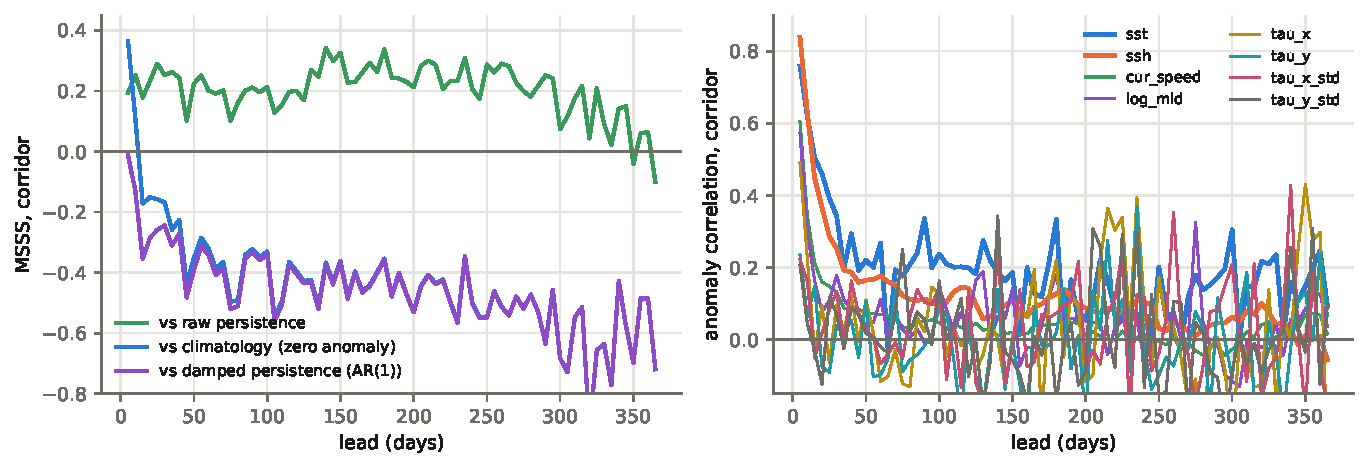
\includegraphics[width=0.94\linewidth]{fig_roll.pdf}
\caption{Left: the rolled head against its three references, corridor
scope. Right: anomaly correlation against lead per scoreable channel; the 32
Argo channels have no scored samples at any lead.\label{fig:roll}}
\end{figure}

\paragraph{The negative score is amplitude, not sign.} For a forecast with
correlation ACC and amplitude ratio $a$ against a zero-anomaly reference,
$\mathrm{MSSS}_{\text{clim}} = 1 - (1 + a^2 - 2a\,\mathrm{ACC})$ identically.
From the head's own per-lead ACC and $a$ this reproduces the 73 measured
values to a mean absolute error of $0.0135$ (Figure~\ref{fig:lim}).
The head emits anomalies at $a\approx0.78$ while its correlation is $0.1$;
rescaled to $a=\mathrm{ACC}$ the same states would score $\mathrm{ACC}^2$ per
lead, a corridor mean of about $+0.02$. Whether a calibration fitted on
training-year starts transfers to held-out starts is untested.

\begin{figure}[t]
\centering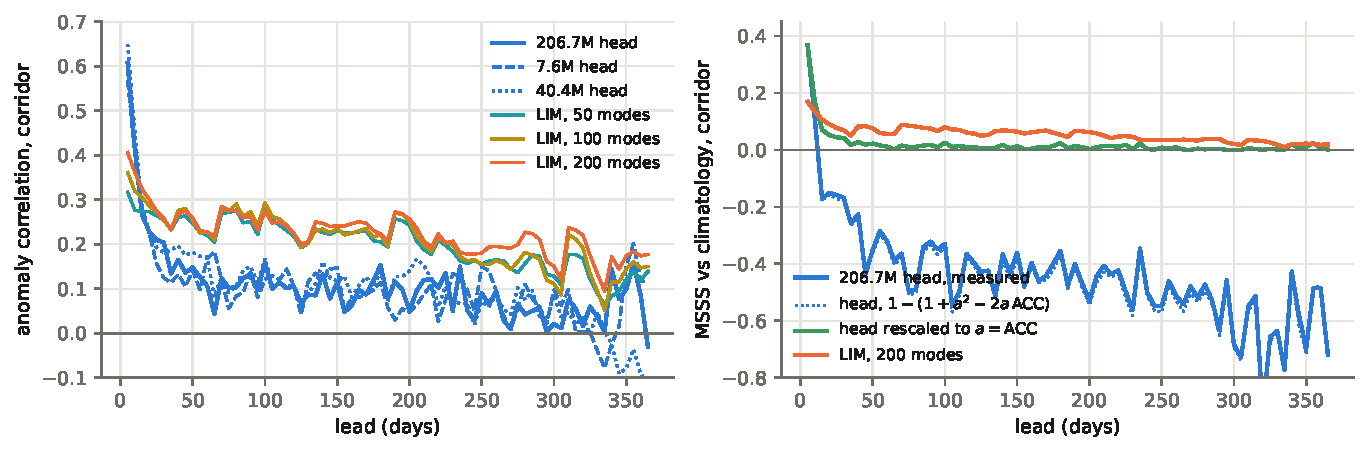
\includegraphics[width=\linewidth]{fig_lim.pdf}
\caption{Left: corridor anomaly correlation per lead for the 206.659M,
40.388M and 7.598M heads and linear inverse models with 50, 100 and 200
modes, from the same starts.
Right: the head's measured $\mathrm{MSSS}_{\text{clim}}$, the value the
identity predicts from its own ACC and $a$, the value the same states would
score at $a=\mathrm{ACC}$, and the 200-mode LIM.\label{fig:lim}}
\end{figure}

\paragraph{A linear inverse model.} A linear inverse model fitted to the
same standardised anomaly field --- the eight scoreable channels over the
window's 86{,}698 ocean pixels, reduced by PCA to $K$ modes, with the
propagator $\mathbf{G}(\tau)=\mathbf{C}(\tau)\mathbf{C}(0)^{-1}$ estimated at
$\tau$ of one pentad from consecutive training bins only --- is rolled from
the same nine starts and scored through the same battery
(Table~\ref{tab:roll}, Figure~\ref{fig:lim}). At 200 modes (76\% of the
training variance; spectral radius $0.986$, leading e-folding time 360 days)
its corridor correlation is $0.41$ at five days, $0.26$ at 90 and $0.18$ at
365; its amplitude falls with lead in step with its correlation, so
$\mathrm{MSSS}_{\text{clim}}$ stays positive at every lead ($+0.17$ at five
days, mean $+0.054$). The head's correlation exceeds the LIM's at five and ten
days only; from fifteen days on the LIM is more correlated with the truth at
every lead, and its mean squared-error score is above both the head's
measured value and the head's amplitude-calibrated value ($+0.019$). Against
damped persistence the LIM loses at leads up to 15 days and wins by
$0.01$--$0.07$ from 30 days out; the head loses at every lead. Fifty and 100
modes score below 200 at every lead (mean correlation $0.200$, $0.209$,
$0.225$). Per channel, the LIM holds sea-surface temperature at $0.48$,
$0.41$, $0.33$ and $0.28$ at 5, 30, 90 and 365 days against the head's
$0.76$, $0.34$, $0.34$ and $0.10$, and sea-surface height at $0.57$, $0.36$,
$0.30$, $0.30$ against $0.84$, $0.25$, $0.11$, $-0.06$. The LIM's training
set is every bin outside a held-out year (2{,}923 bins, 2{,}919 pairs),
which is slightly larger than the pool the head's 144-bin windows admit.

\paragraph{Width on the rolled field.} The 7.598M ($256\times8$) and
40.388M ($512\times12$) heads at their 20{,}000-step end states, rolled
through the identical battery, score the same field as the 206.659M head
(Table~\ref{tab:width}, Figure~\ref{fig:lim}): mean corridor correlation
$0.103$, $0.104$ and $0.105$ across a $27\times$ span in parameters, and
amplitude-calibrated ceilings (mean $\mathrm{ACC}^2$) of $0.018$, $0.022$
and $0.019$. The three differ in amplitude, which is monotone in width
($a = 0.54$, $0.63$, $0.78$) and is the whole of the spread in
$\mathrm{MSSS}_{\text{clim}}$ ($-0.179$, $-0.257$, $-0.439$); the identity
above reproduces each head's 73 leads to a mean absolute error of $0.006$,
$0.007$ and $0.014$. They also differ at the ends of the lead axis. The
40.388M head is the most correlated over the first two pentads ($0.649$ and
$0.452$) and is the only head with a positive $\mathrm{MSSS}_{\text{damped}}$
at any lead ($+0.08$ at five days); the 7.598M head does not decay through
zero, holding $0.10$--$0.14$ from 60 days to a year where the two larger
heads fall to $-0.12$ and $-0.03$, and its $a$ does not grow with lead.
Sea-surface temperature carries the skill in all three (mean
$\mathrm{MSSS}_{\text{clim}}$ $-0.006$, $-0.143$, $-0.165$; positive at 33,
15 and 11 of 73 leads); sea-surface height is the sharpest one-step channel
for all three ($0.87$, $0.87$, $0.84$). All three beat raw persistence at 71
or more of 73 leads, and the linear inverse model is more correlated than
any of them from fifteen days on. The transport bands of the three heads
disagree in sign ($-0.025$, $+0.103$, $-0.244$; $-0.099$, $-0.131$,
$-0.310$; $+0.107$, $-0.242$, $+0.163$). Roll times 7{,}660, 21{,}077 and
77{,}147\,s. One seed each.

\begin{table}[t]
\centering\small\setlength{\tabcolsep}{3.6pt}
\begin{tabular}{r rrr rrr rrr}
\toprule
 & \multicolumn{3}{c}{ACC} & \multicolumn{3}{c}{$\mathrm{MSSS}_{\text{clim}}$} & \multicolumn{3}{c}{$a$} \\
\cmidrule(lr){2-4}\cmidrule(lr){5-7}\cmidrule(lr){8-10}
lead (d) & 7.6M & 40.4M & 206.7M & 7.6M & 40.4M & 206.7M & 7.6M & 40.4M & 206.7M \\
\midrule
5 & $0.569$ & $0.649$ & $0.606$ & $+0.314$ & $+0.422$ & $+0.365$ & $0.69$ & $0.69$ & $0.69$ \\
10 & $0.403$ & $0.452$ & $0.412$ & $+0.125$ & $+0.177$ & $+0.109$ & $0.61$ & $0.63$ & $0.67$ \\
15 & $0.284$ & $0.276$ & $0.265$ & $-0.005$ & $-0.098$ & $-0.172$ & $0.58$ & $0.69$ & $0.76$ \\
30 & $0.124$ & $0.181$ & $0.204$ & $-0.160$ & $-0.123$ & $-0.168$ & $0.55$ & $0.58$ & $0.67$ \\
90 & $0.137$ & $0.150$ & $0.132$ & $-0.120$ & $-0.189$ & $-0.322$ & $0.52$ & $0.62$ & $0.72$ \\
180 & $0.114$ & $0.140$ & $0.153$ & $-0.139$ & $-0.180$ & $-0.354$ & $0.51$ & $0.59$ & $0.78$ \\
365 & $0.119$ & $-0.116$ & $-0.031$ & $-0.181$ & $-0.593$ & $-0.719$ & $0.54$ & $0.66$ & $0.82$ \\
\midrule
mean, 73 leads & $0.103$ & $0.104$ & $0.105$ & $-0.179$ & $-0.257$ & $-0.439$ & $0.54$ & $0.63$ & $0.78$ \\
\bottomrule
\end{tabular}
\caption{The 7.598M, 40.388M and 206.659M heads through the same battery,
corridor scope. Mean $\mathrm{MSSS}_{\text{damped}}$ $-0.200$, $-0.277$ and
$-0.461$; gate/window mean $\mathrm{MSSS}_{\text{clim}}$ $-0.201/-0.213$,
$-0.208/-0.227$ and $-0.395/-0.401$. Single seed each.\label{tab:width}}
\end{table}

\paragraph{Per channel.} Only eight of the forty channels are scoreable.
Sea-surface temperature holds correlation longest ($0.76$ at five days,
$0.34$ at 30 and at 90) and is the only channel whose
$\mathrm{MSSS}_{\text{clim}}$ stays positive beyond a few pentads;
sea-surface height is sharpest at one step ($0.84$) and below $0.2$ by a
month; current speed and mixed-layer depth are one-step quantities; the four
wind channels are noise past one step (Table~\ref{tab:channels}).

\begin{table}[t]
\centering\small
\begin{tabular}{lrrrrr}
\toprule
channel & ACC 5\,d & ACC 30\,d & ACC 90\,d & mean $\mathrm{MSSS}_{\text{clim}}$ & mean $\mathrm{MSSS}_{\text{damped}}$ \\
\midrule
\texttt{sst} & $0.759$ & $0.343$ & $0.337$ & $-0.165$ & $-0.191$ \\
\texttt{ssh} & $0.838$ & $0.252$ & $0.113$ & $-0.499$ & $-0.562$ \\
\texttt{cur\_speed} & $0.604$ & $0.131$ & $0.052$ & $-0.591$ & $-0.606$ \\
\texttt{log\_mld} & $0.572$ & $0.178$ & $-0.009$ & $-0.464$ & $-0.469$ \\
\texttt{tau\_x} & $0.490$ & $0.097$ & $0.022$ & $-0.383$ & $-0.386$ \\
\texttt{tau\_y} & $0.235$ & $0.039$ & $-0.017$ & $-0.426$ & $-0.428$ \\
\texttt{tau\_x\_std} & $0.222$ & $0.134$ & $0.104$ & $-0.409$ & $-0.410$ \\
\texttt{tau\_y\_std} & $0.207$ & $0.070$ & $0.057$ & $-0.465$ & $-0.466$ \\
\bottomrule
\end{tabular}
\caption{Per-channel corridor scores of the rolled head.\label{tab:channels}}
\end{table}

\paragraph{Transport.} The unpooled read-out of the rolled section states
against RAPID gives $r=+0.107$ over 5--90 days ($n{=}162$), $-0.242$ over
95--180 ($n{=}129$), $+0.163$ over 185--365 ($n{=}150$). With about nine
effective independent starts these are inside the noise of zero. A separate
36-month free run from a context ending 2004-12 --- inside the training
years, so not a skill measurement --- correlates $0.636$ with the true
transport at pentad resolution and $-0.13$ on an 18-month low-pass at 61\%
amplitude: what the head tracks lives at high frequency, and the multi-year
band is not measured by this roll.

\paragraph{Statistical power.} The pool has 2{,}417 distinct end-times;
consecutive windows share 143 of 144 frames, and every pixel is a correlated
view of the same temporal patterns. With 206M parameters that is $\sim$85{,}000
parameters per pattern, and the training loss falling long after the
held-out loss has turned is the expected consequence. For field-level scores
the effective sample count is in the thousands and differences can be
resolved; for the transport target (RAPID $\sim$20 years, anomalies
decorrelating over months to years) it is of order ten, and a band
correlation of $\pm0.2$ cannot be. Every rolled number here is one seed;
rolled skill at this cadence has not been replicated, and no two rolled
numbers can yet be called different.

\section{A cone-based design for the next codec and forecaster}\label{sec:design}

The measurements above fix what a redesign has to answer. The codec is at
parity with the raw fields it compresses for a current-state read-out, so its
only value is as a substrate for a forecaster (\S\ref{sec:codec}); the
forecaster learns what transfers inside two thousand steps at every width,
memorises afterwards, emits anomalies whose amplitude does not fall with its
correlation, loses to a damped-persistence null at every lead and to a
200-mode linear inverse model from fifteen days on (\S\ref{sec:stage2}); and
the field, not the transport index, is the only instrument that can resolve
a design choice (nine effective starts at $26.5^\circ$N). This section
specifies both stages from those constraints. Nothing in it has been trained;
every number that is a choice is marked as one, and \S\ref{sec:design-tests}
names the comparison that would settle it.

\paragraph{Both stages read the same shape.} A pixel's future depends on a
cone in space--time: a driver moving at speed $v$ reaches the anchor from
within a distance $v\,\Delta t$ after $\Delta t$, so the set of
space--time points that can bear on the anchor widens into the past, and,
by the same argument run forward, the set the anchor can bear on widens into
the future. Both stages sample that double cone --- an hourglass with the
present at its waist --- and differ only in what fills it and at what scale
(Figure~\ref{fig:hourglass}). Stage 1 reads raw values over the last 30 days
and writes one embedding per cell and pentad; stage 2 reads those
embeddings over the last two years and writes the embeddings of the next
year. In both, the past half of the hourglass is input and never a forecast
target, the waist is the present, and the future half is target only.

\begin{figure}[t]
\centering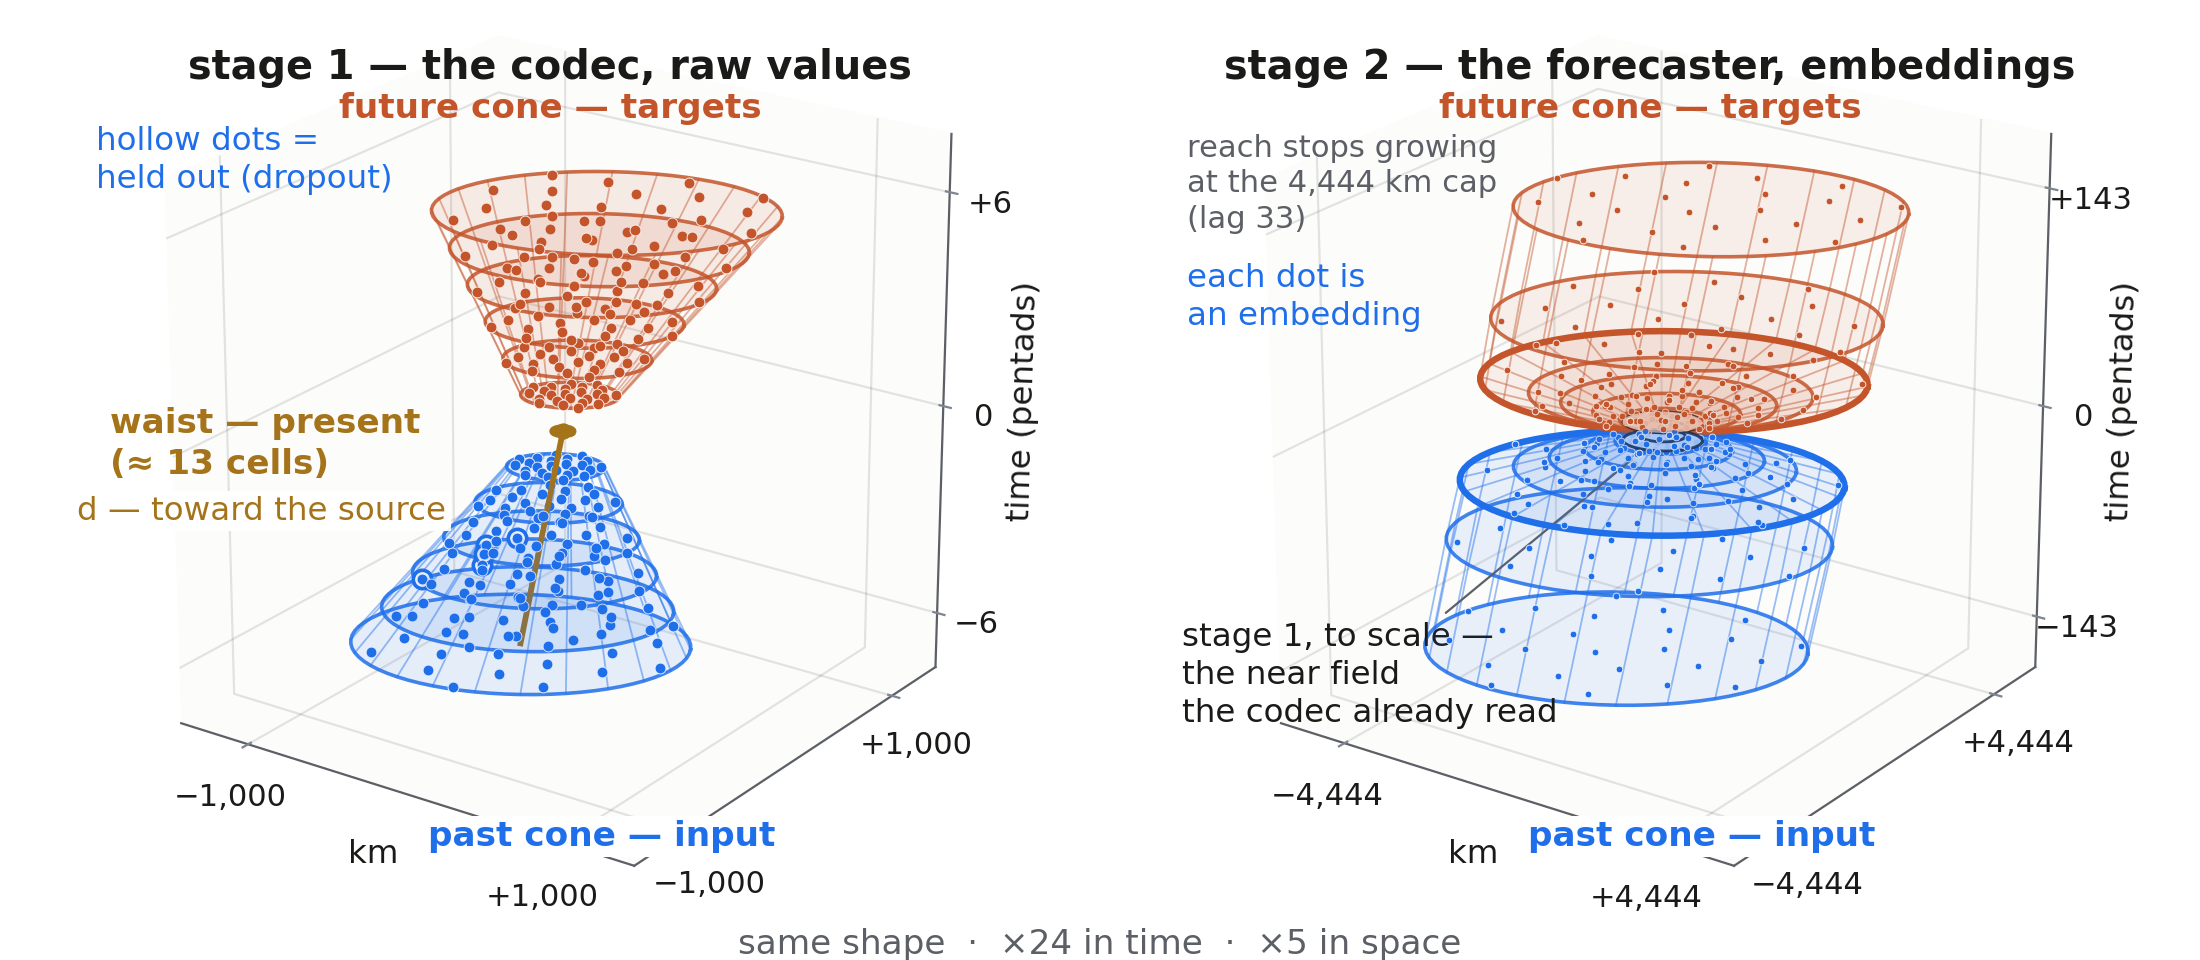
\includegraphics[width=\linewidth]{fig_hourglass.png}
\caption{The hourglass at both scales. Each lag is a footprint of 24
sampling points (a Vogel sunflower, phase-rotated by the golden angle per
lag so consecutive slices interleave) inside an ellipse whose size grows
with lag. Left: stage 1 over raw values, six pentads each way, ${\approx}$900
km at six pentads for the ocean-surface channels, a waist of thirteen
cells. Right: stage 2 over stage-1 embeddings, 7--143 pentads each way,
opening to a 4{,}444 km cap; stage 1's whole hourglass is the small solid at
the centre, the near field the codec has already read.\label{fig:hourglass}}
\end{figure}

\subsection{Data and tokens}\label{sec:design-data}

\paragraph{Grid.} The global $0.25^\circ$ pentad tensor ($721\times1{,}440$
cells, 1982--2024, 3{,}142 bins) in its four native-resolution groups: 7
ocean channels at $0.25^\circ$ (current speed and its two components,
sea-surface height, sea-surface temperature, sea-ice concentration, log
mixed-layer depth), surface chlorophyll-a at $0.25^\circ$ from late 1997,
15 atmosphere-and-land channels at $1^\circ$ (wind stress and its
within-pentad variability, 2\,m air and skin temperature, 10\,m wind,
surface pressure, precipitation, snow water equivalent, soil moisture and
temperature, the two turbulent heat fluxes), and 32 ocean-interior channels
at $1^\circ$ and monthly cadence (temperature and salinity at 16 pressure
levels), with two statics (surface class --- ocean, land, ice sheet, inland
water --- and elevation). A coarse channel is read at its own cell, so nine fine cells
under one $1^\circ$ cell see one number; that is the model's honest view and
is not interpolated. No channel is masked by sphere: a land cell reads its
skin and air temperature and soil state, an ocean cell its surface fields,
and every cell reads the shared atmosphere.

\paragraph{Anomalies and scaling.} Every channel enters as a standardised
anomaly against a day-of-year harmonic climatology (annual and semi-annual
terms) fitted on training years only, divided by a training-year standard
deviation per channel; nothing in the climatology, the scale or the
normalisation of any read-out sees a held-out year. Log-normal quantities
(mixed-layer depth, chlorophyll, precipitation, snow water equivalent) are
transformed before standardisation; bounded fractions (sea-ice
concentration, soil moisture) through a logit. A value that does not exist at that cell and bin --- a land cell's
sea-surface temperature, a month without an Argo profile --- is not a zero:
each token carries an \emph{observed} flag per channel, and an unobserved
entry is masked from the loss and from the encoder's input.

\paragraph{Per-location tokens.} The unit the encoder attends over is a
place at a time: one token per sampled cell and lag carrying the value
vector of every channel present there, the observed-flag vector, the
offset $(\Delta x, \Delta y, \Delta t)$ from the anchor in kilometres and
pentads, a sphere code, the local day-of-year harmonics and the latitude.
One token per dot, not one per channel per dot: the channel dimension lives
inside the token, so the token count is the geometry's and not the
channel count's, and adding a channel costs a vector entry rather than a
token.

\paragraph{Point observations.} Measurements that are not on the grid ---
Argo profiles, surface drifters, moored buoys, along-track altimetry,
surface-ocean carbon samples --- enter as tokens of the same schema placed
where and when they were observed: value, offset from the anchor, a
footprint (the measurement's own spatial and temporal extent), instrument
and channel identifiers. The $k$ nearest profiles in space--time within the
cone are read, $k$ small (three to eight per depth group); there is no
ellipse to learn for them, only the attention over what was measured.
Datasets whose licences forbid redistribution are read on the same footing
and never republished.

\subsection{Stage 1: the hourglass codec}\label{sec:design-codec}

\paragraph{Geometry.} The present is a \emph{waist} of about thirteen cells
(a disc of radius two cells at $0.25^\circ$), read and reconstructed, and
the embedding $z$ is written for the anchor at its centre. Gradients need
neighbours: thermal wind and geostrophy are differences across cells, and a
single-cell present cannot hold one. The past cone samples lags 1--6
pentads, every pentad, so the codec owns the last 30 days at full cadence.
At each lag and for each channel group the dense sampling set is a
24-point sunflower mapped through an ellipse of covariance
$\Sigma(\ell) = \Sigma_0 + \ell^2\Sigma_v$ centred at $\ell\,\mathbf{d}$
from the anchor; initial reaches follow the fastest measured signal of the
group (130\,km per pentad for the ocean surface, ${\approx}$900\,km at six
pentads; 500\,km for wind stress within its ten-day memory; the sea-surface
temperature and mixed-layer channels wide at lags 0--1 where the atmosphere
stirs them and then the ocean's growth; 400\,km flat for land, which does
not advect), and a sparse fixed far ring extends every family to the reach
of the fastest signal of its kind at $1.5\times$ a design speed of 5.4\,m/s,
so that a driver is never excluded by construction. The \emph{prediction
cone} is the past cone point-mirrored through the anchor, leads $+1$ to
$+6$ pentads, sampled the same way and used only as targets; the anchor
column is always among them. Each channel reads the group's shared tokens
through its own Gaussian aperture $w_{c,i,\ell} =
\exp(-\tfrac12\,p_i^\top\Sigma_c(\ell)^{-1}p_i)\,\exp(-\ell\Delta t/\tau_c)$
applied to that channel's entries before the projection --- one scale
$s_c$ and one memory $\tau_c$ per channel, one direction per flow --- at
zero extra tokens.

\paragraph{Learnable geometry.} Eight dimensionless numbers per $1^\circ$
cell and channel group are learned: the drift
$\mathbf{d} = \tanh(\mathbf{x})\,v_{\text{design}}\Delta t$, capped at the
design speed by construction, and the two ellipses stored as matrix
logarithms, $S = \log\Sigma = m\mathbf{I} + k\,[\cos2\theta, \sin2\theta;
\sin2\theta, -\cos2\theta]$, so that no parameter is in kilometres, no
angle wraps, and an Adam step of one learning rate moves every radius by
the same fraction of itself whatever its size. The maps are stored as a
coarse $10^\circ$ field plus a $1^\circ$ residual under an L2 and Laplacian
prior, so data-poor cells inherit their neighbourhood. The geometry learns
in two phases: first through the apertures alone over a fixed candidate set
(a log-radial dot set out to the design reach), so the data loader's reads
are regular and never depend on live weights and the gradient on
$\Sigma_0, \Sigma_v, \mathbf{d}, s_c, \tau_c$ is informed by every candidate
at once; then the dense dot table is re-baked from the learned ellipses
every 2{,}000 steps and swapped at an epoch boundary. The far ring is never
gated, target positions carry a stop-gradient, the future cone is tied to
the past cone by the mirror, the evaluation geometry is frozen for every
arm, and the aperture never enters the loss weights: a learnable cone can
otherwise learn to ask easy questions, and each of those rules closes one
way of doing so.

\paragraph{Tasks.} Each training example is one anchor at one bin and draws
one of four tasks: forecast the prediction cone from the waist and the past
cone (share $0.35$); forecast it from the waist alone with the past fully
hidden (0.15), the snapshot twin inside one model, so every run reports
what history buys; nowcast the hidden waist from the past under a dropout
pattern (0.25); and fill in hidden waist cells and hidden past dots from
what remains (0.25). Dropout patterns fire independently: one channel
hidden at the waist, the most recent lags hidden so the model must
extrapolate from stale history, a $90^\circ$ bearing wedge hidden so it
cannot lean on one direction, dots hidden at random to imitate sparse
observation, and, for the nowcast only, the whole waist. The one rule that
is not a knob: a target's channel must be visible somewhere in the input,
at some lag, or the target is unknowable and teaches the model to predict
the mean; the sampler enforces this and the log counts violations
(required zero). Shares are recorded per run and are the first thing the
comparison in \S\ref{sec:design-tests} varies.

\paragraph{Model.} A masked autoencoder in the strict sense: the encoder
sees only visible tokens and visible channel entries, never a placeholder
for a hidden one. The encoder is a transformer over the ${\approx}$300
per-location tokens of one example (Perceiver-style cross-attention into a
fixed latent set when a fixed-size interface is wanted; a plain encoder
with a learned attention pool otherwise), producing $z$ of width
128--256 --- wider than the 32 used above, because the compression the
forecaster needs is in the token count, not in the width, and a narrow
bottleneck was where capacity fights between the waist and the dots showed.
The decoder is query-based and reads $z$ alone: a query is (offset,
channel, sphere, depth, lead), it cross-attends to $z$, and its head emits a
mean and a log-variance per channel group. Because the query carries the
channel and the offset, ``channel $c$ at point $p$ at lead $\ell$'' is one
query, and the same decoder answers a grid cell, a station and a float
profile. A decoder that could also read the encoder's latents would let
$z$ carry nothing; that path is closed.

\paragraph{Objective.} A heteroscedastic Gaussian likelihood per channel
group in its transformed space, in the decoupled form
\[
\mathcal{L} = \|\mu - y\|^2 \;+\; \tfrac12\, e^{-s}\,(y - \mathrm{sg}[\mu])^2 + \tfrac12\, s,
\qquad s = \log\sigma^2,
\]
so the mean is trained by plain squared error --- what the forecaster
consumes and what every score here measures --- while the variance is
trained by the likelihood with the mean detached, which removes the
pathology in which the variance head explains a hard target away instead of
the mean learning it. $s$ is clamped to $[-8, 8]$, the first 2{,}000 steps
run at fixed $\sigma = 1$, and every family --- waist reconstruction, dot
fill-in, each future lead --- is scored against its own predict-the-mean
bar, logged at every evaluation; the bar is what says which family carries
signal, and a family whose held-out error does not fall below it is
reported as carrying none. Channel groups are weighted explicitly in the
loss as a stated choice, never through $\sigma$ as a side effect.

\paragraph{Training stability.} The failure modes that have been measured
each get a guard. Embedding collapse is invisible to reconstruction loss (a
decoder rescales freely), so the effective rank of $z$ over a fixed
held-out batch and a scale-invariant probe correlation are logged at every
evaluation and the run aborts on two consecutive sub-threshold readings; no
quantisation is switched on from a random initialisation, since a lattice
on an untrained encoder collapses within thousands of steps and a lattice
added to a finished continuous codec does not. Inputs are standardised, so
the gradient clip is $1.0$; AdamW with $\beta_2 = 0.95$, weight decay
$0.1$, a 2{,}000-step warm-up and cosine decay to 10\% of peak; bf16 with
fp32 master weights; the geometry parameters get a learning-rate multiplier
of ten (a choice, recorded per run). Training stops at the held-out minimum
with the minimum's step recorded, and no arm runs past four epochs of
anchors. Held-out years are excluded from every window the forward pass can
see --- every past-cone dot, every future-cone target --- and the exclusion
is certified by brute force before training.

\subsection{Stage 2: the forecaster}\label{sec:design-stage2}

\paragraph{Inputs.} Stage-2 tokens are the codec's embeddings: at each
sampled cell and lag, the mean $\mu$ and log-variance $s$ of $z$, the
offset $(\Delta x, \Delta y, \Delta t)$, the statics and the day-of-year
harmonics of that bin. The past cone reads lag 0 (which already summarises
the last 30 days) and log-spaced lags $1, 2, 3, 5, 8, 13, 21, 34, 55, 89,
144$ pentads --- twelve slices instead of 144 --- each with the anchor
column and a 24-dot footprint whose reach follows the fastest slow signal
(planetary waves and gyre adjustment at $0.05$--$0.1$\,m/s: ${\approx}$1{,}000
km at 34 pentads, the 4{,}444\,km cap from about lag 33 on). Dense sampling
where predictability is dense and sparse where it is not is what keeps the
example at ${\approx}$300 tokens rather than 21{,}000; the dense 144-pentad
window is the ablation. The same eight-number learnable geometry applies at
this scale, with its own $1^\circ$ maps and the same guards.

\paragraph{The linear backbone.} The linear inverse model out-forecasts the
learned head from fifteen days on and a damped-persistence null beats it at
every lead. The design therefore makes the learned model a correction to a
linear one rather than a replacement for it. For the anchor column,
\[
\hat{z}_{t+\ell} = \mathbf{G}_\ell\, z_t \;+\; f_\theta(\text{cone}, \ell),
\qquad \mathbf{G}_\ell = \mathbf{U}\,\mathrm{diag}(e^{-\ell/\tau_j})\,\mathbf{U}^{-1},
\]
where $\mathbf{G}_\ell$ is a linear propagator in embedding space with
learned time constants $\tau_j > 0$ --- contractive by construction, so a
free run decays toward climatology rather than drifting --- initialised
from a linear inverse model fitted to the training-year embeddings, and
$f_\theta$ is the transformer over the cone with a zero-initialised output
projection. At step zero the forecaster \emph{is} the embedding-space
linear inverse model; whatever it becomes has to earn its distance from it
on the held-out field. Damped persistence is the diagonal special case and
is reported as its own null.

\paragraph{Direct multi-lead targets.} The target is the mirrored future
cone: the anchor column and its footprint at leads $1, 2, 3, 5, 8, 13, 21,
34, 55, 73$ pentads (73 pentads is one year), each lead a query
$(\Delta x, \Delta y, \ell)$ to the same decoder head, predicted directly
rather than by chaining one-step predictions. A direct forecast at lead
$\ell$ cannot compound its own errors, its amplitude is set by the data at
that lead rather than by an accumulation, and the log spacing puts the
targets where the correlation is still changing. The anchor column is
weighted 1 and the off-anchor footprint 0.25 (a choice); the footprint
targets are what make the prediction a field with coherent advection
rather than a set of independent columns. Leads beyond a year are reached
by feeding the predicted anchor embeddings at leads $1$--$73$ back as the
recent past and querying again --- the multi-year roll is a second mode of
the same model, not its training objective.

\paragraph{Objective and calibration.} The decoupled Gaussian likelihood on
each target embedding, normalised per lead by that lead's predict-the-mean
bar so that every lead counts equally and the long, unpredictable leads do
not dominate the gradient; plus a decoded-space term through the frozen
codec decoder for the scoreable channels at leads 1, 8 and 34 (squared
error against the standardised anomaly, relative to climatology), because
the embedding metric is not the metric the forecast is scored on; plus,
for the multi-year mode, a two-step pushforward term in which the model is
rolled once with a stop-gradient on the first step and scored on the
second, so it learns to correct its own errors without back-propagating
through the roll. Under a squared-error mean the conditional expectation
shrinks toward zero as correlation falls, so amplitude calibration is a
property of the objective at the held-out minimum and not a post-hoc fit;
the anomaly-correlation--amplitude identity of \S\ref{sec:stage2} is
logged per lead as the check that it holds, and a per-lead scaling fitted
on training-year starts is reported as a diagnostic only.

\paragraph{Regularisation and memorisation.} The held-out minimum inside
two thousand steps and the $30\times$ train/held-out gap say the previous
forecaster had ${\sim}85{,}000$ parameters per distinct temporal pattern.
Three things change that. The globe gives every regime of the ocean and
atmosphere as training patterns rather than one basin's; the log-spaced
cone reduces the parameters per example by a factor of seventy; and the
model's free part is a residual on a linear backbone that the data pin
down with far fewer degrees of freedom. On top of these: Gaussian noise on
the input embeddings at $0.7$ of the persistence scale, as in
\S\ref{sec:stage2};
random dropout of past-cone dots; weight decay; early stopping at the
held-out minimum with the step recorded; and, because the model is cheap
at this token count, a seed ensemble of three to five whose spread is the
first probabilistic forecast and whose mean is the deterministic one.

\paragraph{Probabilistic extension.} Once the deterministic level exists, a
shared low-dimensional noise vector per forecast conditions the head so
that samples are coherent across cells and leads; scored by the fair
continuous ranked probability score. Explicit categorical marginals over a
quantised embedding are the alternative where the conditional distribution
is two-humped, which at six to twenty-four months the El Ni\~no index
plausibly is; both are decided on the dense field, never on an index.

\paragraph{Read-outs.} Every quantity of interest is a head on the
predicted embeddings: transport at $26.5^\circ$N through the unpooled
attention head over the section's cells (\S\ref{sec:codec}), trained on
training-year true embeddings and applied to forecasts; the Ni\~no-3.4
index through the same head shape over its box; any channel at any cell
through the codec decoder. The read-out is the cheap, replaceable end of
the system, and none of them is used to choose between models.

\subsection{Evaluation and the comparisons that decide the design}\label{sec:design-tests}

\paragraph{Protocol.} Held-out years 2009, 2017 and 2023 stay held out of
training, of the climatology and of every statistic; a codec and forecaster
trained on $\le 2020$ are scored once on 2021--2024 as a terminal test.
The battery is the one above: for each lead, mean-squared skill against
climatology, raw persistence and damped persistence, anomaly correlation
and amplitude ratio, per channel and per scope, from three starts per
held-out year, with block-bootstrap intervals over starts. The null ladder
beside every read-out is persistence, damped persistence, the linear
inverse model in data space, the linear inverse model in embedding space,
and an analogue (retrieval) forecast; a learned model is reported against
all five. A configuration is compared to another on the dense field; the
transport and index read-outs are downstream checks and cannot resolve a
difference at nine effective starts. The winning configuration of any
comparison is replicated with a second seed before it is written up.

\paragraph{The comparisons, in order.} (1) The hourglass codec against the
current codec, both frozen, both feeding the same forecaster: the one-step
forecast ratio and the future-cone families against their bars. (2) The
learnable geometry: a fixed hourglass, a learned one initialised at the
fixed one, and a learned one whose surface drift is initialised at the
reversed climatological current --- three seeds each, because the read-outs
include a geometric one (at the $26.5^\circ$N array the learned surface
drift should point south-west up the Florida Current, and attention on
deep profiles north, up the deep western boundary current); the learned
arm is adopted if it beats the fixed arm on the future-cone loss at every
lead $\le 3$, paired at all seeds, with the target-variance flag clean,
and if only the primed arm wins the geometry is set from climatology rather
than learned. (3) The forecaster: the linear backbone with a residual
against the same transformer without it; direct multi-lead targets against
one-step autoregression rolled; log-spaced against dense lags; each on the
same codec, the same starts and the same battery. (4) The far ring: the
learned codec without it, which measures whether the ring pays for its
tokens rather than arguing it. Each comparison is one line in a
configuration; none affects the build order, which is geometry, task mix,
aperture gate, parameter maps and harden step, forecaster.

\section{Related work}\label{sec:related}

\paragraph{Observing the overturning.} Continuous measurement of the
Atlantic meridional overturning is two decades old. The RAPID-MOCHA-WBTS
array at $26.5^\circ$N has measured the transport since April 2004 as the
sum of the Florida Current cable, the Ekman transport from wind stress and
the geostrophic interior from boundary density moorings \cite{mccarthy2015};
the record reads $17.0\pm2.8$\,Sv with a trend of $-1.0$ [$-0.4$, $-1.6$]
Sv per decade that is marginally significant and dominated by a 2004--2010
drop and a 2010s pause \cite{mccarthy2025,lee2024}, with the climate signal
carried by the deep and thermocline components rather than by the Gulf
Stream or Ekman terms \cite{mccarthy2025}. The Florida Current itself shows
four decades of steady state once the cable is corrected for geomagnetic
secular variation \cite{volkov2024}. MOVE at $16^\circ$N monitors the deep
western boundary since 2000 \cite{send}; OSNAP measures the subpolar
overturning since 2014 and places most of it east of Greenland
\cite{osnap,fu2025}; a 2026 synthesis of four western-boundary arrays reads a
meridionally consistent decline in deep western transport between
$16.5^\circ$ and $42.5^\circ$N, partly compensated at the eastern boundary
\cite{xing2026}. Whether the overturning weakened before 2004 is contested
between sea-surface-temperature fingerprints \cite{caesar}, which read a
$\sim$15\% decline, and air--sea heat-flux fingerprints, which read none
since the 1960s \cite{terhaar2025}. Our transport target is the RAPID series
deseasonalised at monthly and pentad resolution, with MOVE as a second
target, and our inputs carry no transport measurement.

\paragraph{Reconstructing transport from observables.} The classical line
regresses the $26.5^\circ$N transport on physically chosen observables:
satellite sea level with the cable and Ekman terms \cite{fw2015}, sea level
through a thermal-wind argument \cite{sf2021}, or boundary densities
\cite{worthington}; these reach $r$ of $0.8$--$0.95$ on 18-month low-passed
series with in-sample calibration, and the one out-of-sample case holds out
a single year. The machine-learning line trains on simulations: a
convolutional network reading bottom pressure, sea level, temperature and
wind strips reaches $r\approx0.98$ inside a laminar $1^\circ$ state estimate
\cite{solodoch}, the same task in eddy-resolving models explains
$0.44$--$0.74$ of the variance \cite{meng,woelker}, and a graph network on
Argo profiles, wind stress and the boundary currents trained on VIKING20X
recovers about 80\% of the seasonal variance at $26.5^\circ$N with monthly
errors under 1\,Sv \cite{woelker}; deep-learning reconstructions from surface
fields trained on climate models extend an index back to 1900
\cite{michel2025}. Our read-out differs from all of these in protocol
rather than in method: real RAPID data, monthly or pentad resolution with no
low-pass filter, no transport among the inputs, and a year-blocked k-fold in
which every year is held out in turn. On those terms a frozen embedding
reads transport at $r=0.67$ and a raw-pixel head at $0.66$
(\S\ref{sec:codec}), which is where the eddying-model results place the
difficulty of the task; the same read-outs low-passed at 18 months score
$0.33$--$0.75$ across codec seeds on nine effective points, which is why
the report quotes unfiltered numbers.

\paragraph{Forecasting the overturning.} Initialised decadal prediction
systems show positive skill for subpolar ocean heat content at lead years
2--10 and for coastal sea level along the North American east coast at
3--5 years \cite{yeager2018,carmocosta2025}, but the direct transport record
is too short for the overturning itself to be verified at those leads; at
$26.5^\circ$N the signal-to-noise ratio of the trend is not expected to
exceed 2 before about 2040 \cite{mccarthy2025}. The verification framework
used here --- mean-squared skill scores against climatology and persistence,
anomaly correlation per lead, a damped-persistence reference --- is the one
established for interannual-to-decadal prediction \cite{goddard}. The
linear inverse model \cite{penland} is the standard empirical forecast
against which such systems are judged, including as a benchmark for
decadal forecasts of surface temperature \cite{newman2013}; the version in
\S\ref{sec:stage2} fits it in the same standardised field the transformer is
scored on. Statistical early-warning analyses of sea-surface-temperature
fingerprints have placed a tipping of the overturning in the mid-21st
century \cite{ditlevsen2023}, but the estimate moves by a century or more
with the choice of dataset and fingerprint \cite{benyami2024}, and
physics-based indicators such as the freshwater transport at $34^\circ$S
\cite{vanwesten2024} are the alternative; none of this is a forecast at
the pentad-to-seasonal leads measured here, where the question is whether
any learned model adds to a linear operator.

\paragraph{Learned ocean and climate forecasting.} Neural ocean forecasters
at $1/4^\circ$ to $1/12^\circ$ and the global weather models they descend
from \cite{pangu,graphcast} operate at daily leads on full reanalysis fields
and are cited for orientation; at monthly cadence, convolutional ENSO
forecasts hold Ni\~no3.4 correlation above $0.5$ to about 17 months
\cite{ham} and sea-surface-temperature anomaly fields are forecast to 18
months with recurrent networks \cite{taylorfeng}. Architecturally the codec
is a masked autoencoder \cite{mae} over channel tokens, and the
frozen-representation evaluation used throughout follows the argument that
frozen backbones with shallow read-outs are the honest measure of a
foundation model's representation \cite{lehmann}; the closest statement of
the per-pixel embedding-field idea is terrestrial \cite{alphaearth}.

\section{What the results support}

For the current-state transport read-out the codec is at parity with the raw
fields it compresses; its value, if any, is as a substrate that a
transformer can attend over and roll forward, and on that use the transformer
has learned what it learns inside two thousand steps at any width, rolls
the same field at 7.6M, 40.4M and 206.7M parameters, forecasts sea-surface
temperature and height for days to weeks, does not beat a damped-persistence
null at any lead, and is out-forecast beyond ten days by a linear inverse
model with 200 modes fitted to the same field. The linear
model is therefore the reference against which any further change to the
forecaster is scored: what a learned model adds at leads of one to two
pentads, and whether any change beats the linear model at three. The next
measurements are the ones that bound this further: a retrieval baseline and
a linear inverse model in embedding space through the identical battery,
with block-bootstrap intervals; the early-stopped checkpoints rolled
against the end states shown here; amplitude
calibration fitted on training-year starts; and a codec trained on
$\le 2020$ so that a terminal 2021--2024 test can be run once.
\S\ref{sec:design} is the design these measurements motivate --- the same
hourglass at both stages, a codec that owns the last thirty days of raw
values, and a forecaster that is a residual on the linear model rather than
its replacement --- and \S\ref{sec:design-tests} the comparisons, in
order, that would accept or reject each of its choices.

\begin{thebibliography}{99}\small
\bibitem{mccarthy2015} G. McCarthy et al.\ (2015). Measuring the Atlantic
meridional overturning circulation at 26$^\circ$N. \emph{Progress in
Oceanography} 130.
\bibitem{mccarthy2025} G. McCarthy et al.\ (2025). Signal and noise in the
AMOC at 26$^\circ$N. \emph{Geophysical Research Letters} 52.
\bibitem{lee2024} S.-K. Lee et al.\ (2024). A pause in the weakening of the
Atlantic meridional overturning circulation since the early 2010s.
\emph{Nature Communications} 15.
\bibitem{volkov2024} D. Volkov et al.\ (2024). Florida Current transport
observations reveal four decades of steady state. \emph{Nature
Communications} 15.
\bibitem{send} U. Send, M. Lankhorst, T. Kanzow (2011). Observation of
decadal change in the Atlantic meridional overturning circulation using 10
years of continuous transport data. \emph{Geophysical Research Letters} 38.
\bibitem{osnap} M. S. Lozier et al.\ (2019). A sea change in our view of
overturning in the subpolar North Atlantic. \emph{Science} 363.
\bibitem{fu2025} Y. Fu, M. S. Lozier et al.\ (2025). Characterizing the
interannual variability of North Atlantic subpolar overturning.
\emph{Geophysical Research Letters} 52.
\bibitem{xing2026} X. Xing, S. Elipot, W. Johns, D. Smeed, B. Moat,
J. Loder (2026). Meridionally consistent decline in the observed western
boundary contribution to the AMOC. \emph{Science Advances} 12.
\bibitem{caesar} L. Caesar et al.\ (2018). Observed fingerprint of a
weakening Atlantic Ocean overturning circulation. \emph{Nature} 556.
\bibitem{terhaar2025} J. Terhaar, L. Vogt, N. Foukal (2025). Atlantic
overturning inferred from air--sea heat fluxes indicates no decline since
the 1960s. \emph{Nature Communications} 16.
\bibitem{fw2015} E. Frajka-Williams (2015). Estimating the Atlantic
overturning at 26$^\circ$N using satellite altimetry and cable measurements.
\emph{Geophysical Research Letters} 42.
\bibitem{sf2021} A. Sanchez-Franks et al.\ (2021). A dynamically based
method for estimating the AMOC at 26$^\circ$N from satellite altimetry.
\emph{Ocean Science} 17.
\bibitem{worthington} E. Worthington et al.\ (2021). A 30-year
reconstruction of the Atlantic meridional overturning circulation shows no
decline. \emph{Ocean Science} 17.
\bibitem{solodoch} A. Solodoch et al.\ (2023). Machine learning-derived
inference of the meridional overturning circulation from satellite-observable
variables. \emph{JAMES} 15.
\bibitem{meng} Y. Meng et al.\ (2024). Circumpolar transport and overturning
strength inferred from satellite observables using deep learning.
\emph{JAMES} 16.
\bibitem{woelker} E. W\"olker, W. Rath, M. Renz, A. Biastoch (2025).
Estimating the AMOC from Argo profiles with machine learning trained on
ocean simulations. \emph{Ocean Science} 21.
\bibitem{michel2025} S. Michel et al.\ (2025). Deep-learning reconstructions
of the Atlantic meridional overturning circulation since 1900.
\emph{Environmental Research Letters} 20.
\bibitem{yeager2018} S. Yeager et al.\ (2018). Predicting near-term changes
in the Earth system: a large ensemble of initialized decadal prediction
simulations using the Community Earth System Model. \emph{BAMS} 99.
\bibitem{carmocosta2025} T. Carmo-Costa et al.\ (2025). Decadal prediction
skill of North Atlantic ocean heat content in CMIP6 systems. \emph{Earth
System Dynamics} 16.
\bibitem{goddard} L. Goddard et al.\ (2013). A verification framework for
interannual-to-decadal predictions experiments. \emph{Climate Dynamics} 40.
\bibitem{penland} C. Penland, P. Sardeshmukh (1995). The optimal growth of
tropical sea surface temperature anomalies. \emph{Journal of Climate} 8.
\bibitem{newman2013} M. Newman (2013). An empirical benchmark for decadal
forecasts of global surface temperature anomalies. \emph{Journal of Climate}
26.
\bibitem{ditlevsen2023} P. Ditlevsen, S. Ditlevsen (2023). Warning of a
forthcoming collapse of the Atlantic meridional overturning circulation.
\emph{Nature Communications} 14.
\bibitem{benyami2024} M. Ben-Yami et al.\ (2024). Uncertainties too large to
predict tipping times of major Earth system components from historical data.
\emph{Science Advances} 10.
\bibitem{vanwesten2024} R. van Westen, M. Kliphuis, H. Dijkstra (2024).
Physics-based early warning signal shows that AMOC is on tipping course.
\emph{Science Advances} 10.
\bibitem{pangu} K. Bi et al.\ (2023). Accurate medium-range global weather
forecasting with 3D neural networks. \emph{Nature} 619.
\bibitem{graphcast} R. Lam et al.\ (2023). Learning skillful medium-range
global weather forecasting. \emph{Science} 382.
\bibitem{ham} Y.-G. Ham, J.-H. Kim, J.-J. Luo (2019). Deep learning for
multi-year ENSO forecasts. \emph{Nature} 573.
\bibitem{taylorfeng} J. Taylor, M. Feng (2022). A deep learning model for
forecasting global monthly mean sea surface temperature anomalies.
\emph{Frontiers in Climate} 4.
\bibitem{mae} K. He et al.\ (2022). Masked autoencoders are scalable vision
learners. \emph{CVPR}.
\bibitem{lehmann} F. Lehmann et al.\ (2026). Frozen foundation-model
backbones with shallow decoders as an evaluation standard. \emph{JGR
Machine Learning and Computation}.
\bibitem{alphaearth} C. Brown, M. Kazmierski, V. Pasquarella et al.\ (2025).
AlphaEarth Foundations: an embedding field model for accurate and efficient
global mapping from sparse label data. arXiv:2507.22291.
\end{thebibliography}

\appendix
\section{Data and code availability}\label{app:avail}

\begin{sloppypar}
Code: \url{https://github.com/blauewelt/earth} (codec trainer
\path{ml/train.py}, stage-2 trainer \path{ml/temporal.py} and its JAX
port \path{ml/jaxport/}, evaluator \path{ml/rollout_spatial.py}). Result
bundles are on the repository's \path{ml-metrics} branch
(\path{probes-<n>.json}; the rolls here are \path{probes-516.json}, \path{probes-520.json} and \path{probes-523.json}, the linear inverse model \path{probes-527.json} (\path{ml/lim_baseline.py}), the
codec probe ladder is in the bundles named in \path{ml/EXPERIMENTS.md}).
Weights are on the \path{model-checkpoints-v1} release
(\path{run-415__pixelmae.pt}; \path{head-weights-e059-200k-window-s0.pt}
and the \path{e060a}/\path{e060b} heads named likewise); the
tensor on the \path{data-cache-v1} release and the Hugging Face dataset
\path{chfrank/earth-tensors}; the codec's embedding of it on
\path{embed-cache-v1}. Stage-2 figures and tables are generated by
\path{ml/paper/make_figs.py} from \path{ml/paper/data/report_data.json}, built by \path{ml/paper/extract_data.py} from those bundles and the
training records; codec probe numbers are transcribed from the archived
per-run bundles, with the source named beside each in the figure script.
\end{sloppypar}

Sources: GLORYS12 and the GREP ensemble (E.U.\ Copernicus Marine Service
Information, used under the CMEMS licence with credit to the service); the
Roemmich--Gilson Argo climatology (Scripps; Argo data are collected and made
freely available by the International Argo Program and the national programs
that contribute to it); NCEP/NCAR Reanalysis-1 (NOAA PSL); OISST v2.1 (NOAA
NCEI); the RAPID-MOCHA-WBTS transport time series (NERC, NSF, NOAA); the MOVE
transport time series (NOAA).

\end{document}
